\section{Introduction}
\subsection{Motivation}
Assistive robots in domestic environments have the potential to aid persons with special needs in their daily living, thereby helping them to maintain a quality of life that would otherwise be lost.
Robotic assistance can be beneficial to a variety of domains and users: the care and assistance of the elderly at home or in a nursing environment, assistance of persons with physical impairments and persons with cognitive or social deficits such as dementia or autism spectrum disorder.

The Department of Economic and Social Affairs of the United Nations estimates that the number of people in Germany above an age of 70 years will leap from 13 to 19 million, i.e. increase by around $46\%$ over the next 20 years (see figure \ref{fig:population_germany}).
With the world's population growing older and caring facilities having reached their capacities already today, the need for assistive systems is specifically critical in elderly care.
Domestic robots may provide the freedom to keep living in the own home, prolong the time before living in a nursing environment becomes necessary and thereby relieve take the load off such institutions.

\begin{figure}[H]
    \centering
    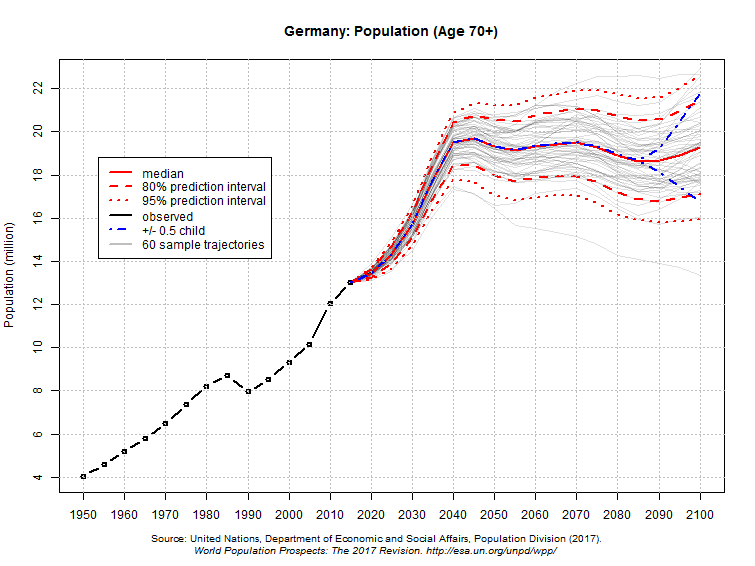
\includegraphics[width=\textwidth]{img_introduction/Germany.png}
    \caption{Estimation of the population of age 70+ in Germany}
    \label{fig:population_germany}
\end{figure}

Contact assistive robotics, i.e. robots with the ability to manipulate objects in their environment offer to perform simple every-day tasks for the physically impaired, the elderly and people in general need of help.
One of the biggest concerns in assistive robotics is inadvertently harming a user\cite{mataric_socially_2016}.
Robots equipped with manipulators, which represent additional powerful hardware, may raise the concern of possible harm and therefore struggle against widespread acceptance in elderly care or private homes.

In contrast, the field of socially assistive robotics aims at assisting persons through social rather than physical interaction\cite{feil-seifer_defining_2005}.
Examples include robotic animal toys, which intends to improve the physiological as well as psychological fitness of elderly persons through robotic interaction.
A prominent example is the robotic seal PARO\cite{wada_analysis_2002}, which targets at providing the social benefits of a pet without the usual occurring responsibilities.
Socially assistive robots have since been extended to a variety of helpful functions, such as intelligent reminding, cognitive stimulation and mobile videophony\cite{gross_progress_2011}.

This work is carried out in the context of the RoboLand project\footnote{\url{www.roboland-projekt.de}}, which aims at increasing social interactions for elderly persons with dementia in rural regions through telepresence.
Telepresence is an extended form of videophony through a remote controlled robot.
The market research institute \textit{Wainhouse Research} defines telepresence as ``a videoconferencing experience that creates the illusion that the remote participants are in the same room with you''\cite{davis_telepresence_2007}.
The underlying hypothesis of the RoboLand project is, that telepresence can have the biggest social impact in rural environments, where relatives live far from family members with cognitive impairments and visiting regularly is difficult.

Current telepresence robots span a wide spectrum of capabilities.
The initial two models that were selected for practical evaluation in the RoboLand project are:
\begin{description}
    \item[Double] \hfill\\
    A remote controlled self-balancing platform with an iPad attached to a telescopic extendable shaft.\footnote{\url{www.doublerobotics.com}} 
    \item[Amy] \hfill\\
    A ROS-based\footnote{\url{www.ros.org}} robotic platform, designed for telepresence and social assistance.
    In contrast to \textit{Double}, \textit{Amy} is equipped with a variety of additional sensors such as ultrasonic sensors, infrared sensors, an inertial measurement unit, a 2D camera and a 3D camera.\footnote{\url{www.amyrobotics.com}}
    Amy is therefore equipped to perform autonomous robotics tasks such as navigation, mapping and recognition of persons or objects.
\end{description}


\subsection{Scope of this Work}
In order to provide assistance in a domestic environment, an autonomous assistive system first needs to know in what form and when assistance is required.
This can either be achieved by registering direct commands from the user, e.g. through voice recognition and touchscreen inputs or by autonomous recognition of visual stimuli from the system's environment.
By autonomously recognizing situations in which assistance is required, a robotic system is able to then offer a set of actions which could be executed to assist.
This provides a form of social immersion of the robot, since it is actively able to engage the user and offer assistance even if it might not actually be required. 

The underlying hypothesis of this work is that currently performed actions by a human user are the best indicator of whether assistance is required or human-robot communication should be initiated.
This work therefore aims at providing a basis for improving assistive robotics through human action recognition from video data by an adapted deep learning approach, specifically targeted against the recognition of daily-living actions.

Since video cameras are a widespread and cheap technology, available in every mobile phone and naturally available in telepresence robots, a vast amount of video data for training action recognition algorithms is easily obtainable from online video platforms such as YouTube.
An action recognition system that processes 2D video-data can therefore be easily deployed, since regular 2D cameras form the standard equipment of most robots.
In the context of the RoboLand project, we aim at extending the deployed robots beyond the telepresence functionality towards social assistance through human action recognition.

Action recognition is a classification task.
An action recognition system is presented with a video, usually a short clip that contains the performance of a single action, and then outputs the corresponding action class according to a finite and predefined set of recognizable actions.
In learning systems, this set of recognizable actions is defined by the labelling of the dataset that was used to train the system.
A properly labelled and big dataset is therefore vital for successfully training an action recognition system.

Deep learning approaches have shown remarkable results in a multitude of vision tasks.
These include handwritten digit recognition\cite{lecun_handwritten_1990}, object detection and recognition\cite{redmon_you_2016}\cite{ren_faster_2015} and scene segmentation\cite{chen_deeplab:_2016}.
In our previously conducted literature survey\cite{schobel_evaluation_2017}, the performance of deep learning approaches in action recognition has been compared to the classical method of using hand-crafted features.
In that work we concluded that deep learning approaches do not yet outperform state-of-the-art hand-crafted feature methods, but show promising and competitive results.
We therefore aim at increasing the performance of a deep learning approach for action recognition and specifically train a system for recognizing daily-living actions, which could be deployed on an assistive robotic system in the real-world.

\subsection{Challenges}
The practical value of an action recognition system heavily depends on the data, that was used for training it, since the dataset defines the action classes that can later be recognised;
therefore, a sufficiently large dataset of daily-living actions is necessary to obtain a classifier that can be used for recognising daily-living actions in a real-world setting.
The common disadvantage of deep neural networks, namely that they require a lot of labelled data in order to generalize effectively, has to be addressed.
Since manually collecting and labelling video data is expensive, action recognition datasets are usually sampled from sources like movies, television broadcasts or online video platforms\cite{hassner_critical_2013}.
These videos however are often biased towards unrealistic or entertaining videos in staged and uncommon settings.
Traditionally, sports video have been used for general action recognition benchmarking datasets, since sports videos are widely distributed and a distinct label is easily obtainable.

Fortunately, the work of \textcite{sigurdsson_hollywood_2016} already addressed the challenge of obtaining a dataset with \textit{boring} daily-living actions.
Since these types of actions are hard to sample from movies or the internet, a series of crowdsourced tasks was deployed to compile the dataset called Charades\cite{sigurdsson_hollywood_2016}.
The complete process of creating actions scripts, recording the videos and annotating them with action labels was done by 267 individuals from three different continents.
The videos in the Charades dataset were recorded in regular homes by a decently large number of private actors.
The dataset thus contains a decent amount of variety in action performances in real-world scenes.
In particular 9,848 videos with 66,500 individually labelled and temporally localized action instances are contained in the dataset, as it is specifically designed to enable robotic applications in real-world environments.

The size of 66,500 action instances is extremely small for a deep learning dataset, since deep learning architectures usually require more data.
In comparison, the two currently biggest action recognition datasets are Sports-1M\cite{karpathy_large-scale_2014} (around one million noisily labelled sports videos) and YouTube-8M\cite{abu-el-haija_youtube-8m:_2016} (around eight million noisily labelled YouTube videos).
The practical benefit of these datasets however is questionable, since the labels are noisy and the contained actions are not temporally localized.
Recently, the Kinetics dataset was published, which addresses the issues of action recognition datasets being too small by providing  videos.
The actions in Kinetics are comparably well localized, since each video has a fixed length of 10 seconds which contains the action.
Even these datasets are magnitudes smaller compared to common image classification datasets, such as ImageNet\cite{deng_imagenet:_2009} with a total number of $14,197,122$ images or the 80 million tiny images dataset\cite{torralba_80_2008} with $79,302,017$ images.

In addition to generally smaller dataset sizes, processing video data yields further challenges not present in the domain of image processing.
Since multiple frames are being processed per training step, a single video input has a higher dimensionality than an image input by a factor according to the number of processed frames per iteration.
This leads to bigger sizes of individual inputs and therefore smaller batch sizes, i.e the number of inputs processable per training step, need to be incorporated to not exceed memory limitations.

Furthermore, videos are encoded in order to decrease file-sizes for distributing them.
Since pre-decoding and storing raw RGB frames would have exceeded our storage capacities, a partial decoding step has to be incorporated into the data-preprocessing pipeline for network input generation.
This adds to the time until an input is ready to be further processed and potentially, if not handled otherwise, delays the overall training process.


\subsection{Methodology}
In deep learning for action recognition, two main approaches can be identified:
\begin{enumerate}
    \item
    Extending the convolutional kernels in regular (2D) CNNs to the temporal dimension and thereby enabling them to process 3D video volumes that result from stacking consecutive video frames.
    One of the first publications that incorporate 3D CNNs for action recognition is \cite{ji_3d_2013}.
    \item
    Incorporation of two separated processing streams of 2D CNNs into the overall network architecture. A spatial recognition stream processes RGB video frames and an additional temporal recognition stream receives optical flow inputs to incorporate explicit motion information. The prototypical publication that describes this approach is \cite{simonyan_two-stream_2014}.
\end{enumerate}

Our previously conducted survey\cite{schobel_evaluation_2017} concludes that the two-stream approach in general performs better, than single-stream 3D convolutional networks.
The major deficiency of 3D convolutional neural networks is that they treat the temporal and spatial domain equally:
a video volume of stacked input frames is treated as a regular 3D object.
However, the temporal dimension is not inherently equal to the spatial dimension since adjacent frames correlate by obeying the laws of physics, i.e. shown objects cannot instantaneously disappear but instead move with finite velocities, so that the amount of change between frames is limited.

To address the above stated challenges, we incorporate an unsupervised pre-training strategy called \textit{temporal order verification}, which has previously shown to increase performance of 2D CNNs in action recognition.
During pre-training with \textit{temporal order verification}, a model has to determine whether a presented input is in correct or incorrect order.
These inputs can be sampled from source videos by creating network inputs from the video frames and possibly permuting them.
This is in the strictest sense a supervised pre-training strategy;
however, since the labels \textit{correct temporal order} and \textit{incorrect temporal order} are automatically determined, it is treated as an unsupervised method.
The obtained model weights are then used as initialization for training on the actual labelled dataset.

Pre-training a model with \textit{temporal order verification} has the following beneficial properties, which makes it particularly interesting for our work.
\begin{itemize}
    \item 
    since it is a quasi unsupervised pre-training strategy, large amounts of possibly unlabelled video data can be incorporated in the pre-training process.
    \item
    \textcite{misra_shuffle_2016} describe the benefit of \textit{temporal order verification} in that the network needs to reason about the movement in the presented inputs, in order to determine the temporal order.
    The learned representations, therefore need to encode motion of the inputs, which is highly informative for the presented actions.
\end{itemize}

In this work, we investigate the transfer of this pre-training strategy to a 3D CNN model, namely the \textit{C3D} convolutional network as described in \cite{tran_learning_2015}.
Our working hypothesis is that \textit{temporal order verification} is especially beneficial for a single-stream 3D CNN in the domain of daily-living action recognition because:
\begin{enumerate}
    \item
    There is not much labelled training data available that features \textit{boring} daily-living actions in real-world environments and incorporating an unsupervised pre-training strategy addresses this problem.
    Specifically, the benefit of using the Kinetics dataset for pre-training is evaluated.
    \item 
    \textit{Temporal order verification} has shown to result in input representations that focus on human motion by comparing the temporal relations between inputs.
\end{enumerate}

To address the problem of pre-processing times, we implement a high performant multi-threaded input pipeline, that decodes and prepares network inputs in parallel.
According to the available hardware, an arbitrary number of threads can feed the prepared network inputs into a FIFO-queue for training.
To address the problem of small batch-sizes, we incorporate a multi-GPU setup for training in which several GPUs process individual batches. Averaging of the gradients per GPU results in an effectively bigger batch size.


\newpage
\section{Related Work}
The field of action recognition from video can broadly be divided into two main approach classes:
\begin{description}
    \item[Hand-crafted feature based approaches] \hfill \\
    These video classification algorithms extract video/image features around previously identified areas of motion from an input video.
    These features are aggregated into a fixed-length representation of the video and then classified using an arbitrary classifier.
    The performance of these approaches is heavily influenced by \textit{where} features are extracted and \textit{what} kind of features are being extracted.
    Interest-point detectors and feature extractors are carefully hand-crafted for that purpose.
    Although hand-crafted feature based approaches yield competitive results in action recognition, the results of \textcite{wang_evaluation_2009} indicate, that there is no universally best manually engineered set of features for all tasks.
    \item[Deep Learning based approaches] \hfill \\
    (Deep) Learning approaches eliminate the need of manual feature engineering by learning to extract descriptive features and video representation directly from training data.
    Deep models are end-to-end trainable, i.e. once a model architecture is constructed it requires a large amount of labeled training videos to learn the direct correspondence between action label and input data.
\end{description}


\subsection{Hand-Crafted Feature-based Approaches}
The research interest in human action recognition, fuelled by the amount of possible applications, has produced a decent number of comprehensive survey articles about human action recognition approaches with hand-crafted features and deep learning
\cite{poppe_survey_2010, aggarwal_human_2011, chaquet_survey_2013, langkvist_review_2014, herath_going_2016, kang_review_2016}.
This section provides a very brief overview of the main ideas behind using hand-crafted feature based methods.
For a detailed review we refer the reader to the article of \textcite{poppe_survey_2010}.


In the class of \textit{space-time volume} approaches, a global video representation is built from the complete input video.
The input video is thereby interpreted as a 3D space-time volume, which results from stacking the individual video frames.
These approaches use template matching to compare the representation of an to be classified input video with a previously created template that represents the input class.
 
\textcite{bobick_recognition_2001} create video representations by overlying the foreground silhouettes of the person performing action.
Treating each silhouette as equally important results in the binary motion-energy image.
Letting the silhouettes decay over time results in the scalar valued motion-histogram image, as displayed in figure \ref{fig:spacetimevolumes_meimhi}.

\begin{figure}[H]
    \centering
    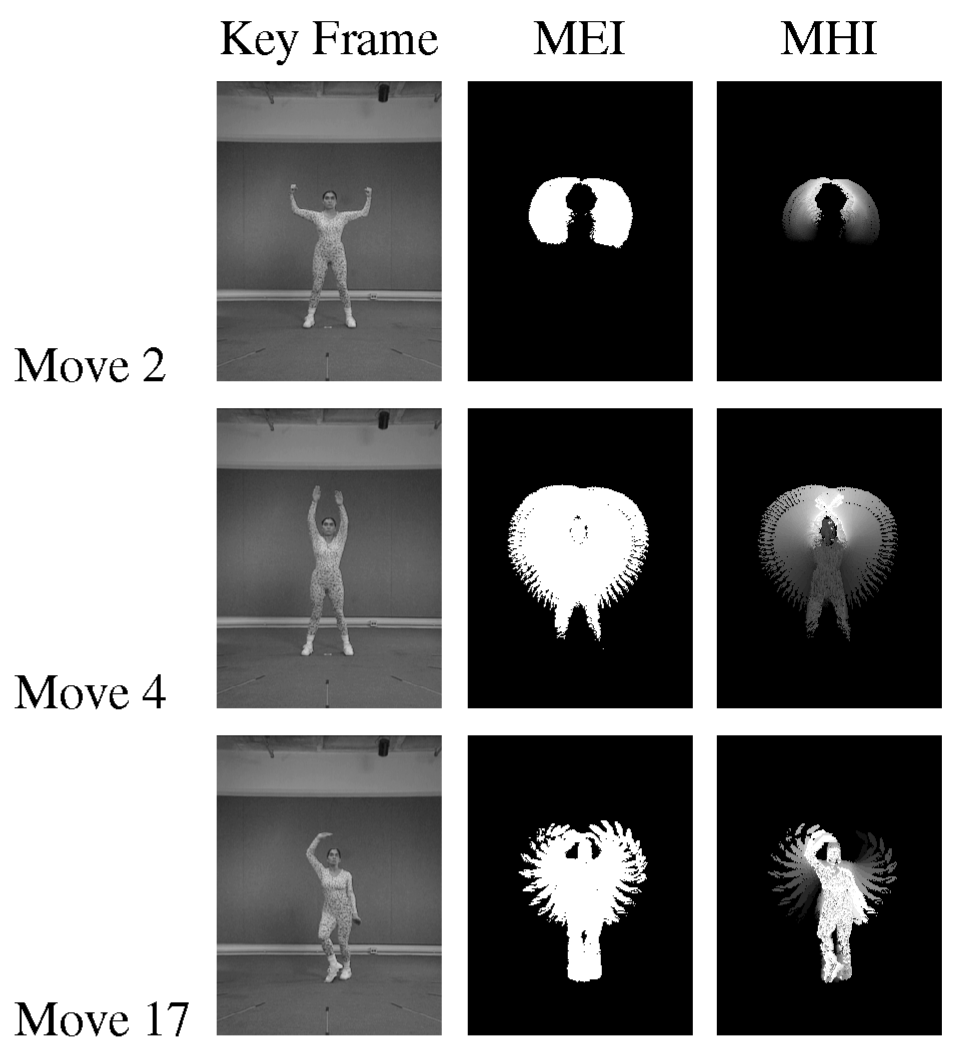
\includegraphics[width=.45\textwidth]{img_related/spacetimevolumes_meimhi}
    \caption{\textit{(left)} Example frames of three videos showing different ballet moves. \textit{(middle)} Motion-energy image (MEI). \textit{(right)} Motion-history image (MHI) \cite{bobick_recognition_2001}}
    \label{fig:spacetimevolumes_meimhi}
\end{figure}

The main idea of \textit{trajectory-based} approaches is that the trajectories of a persons tracked joints provide informative to recognize the displayed action.
The resulting joint trajectories can either be compared directly by template matching or trajectory can be extracted to be classified.
\textcite{sheikh_exploring_2005} track $13$ joint positions and use the resulting trajectories for action recognition.
The approach is illustrated in figure \ref{fig:trajectories_sheikh}.

\begin{figure}[H]
    \centering
    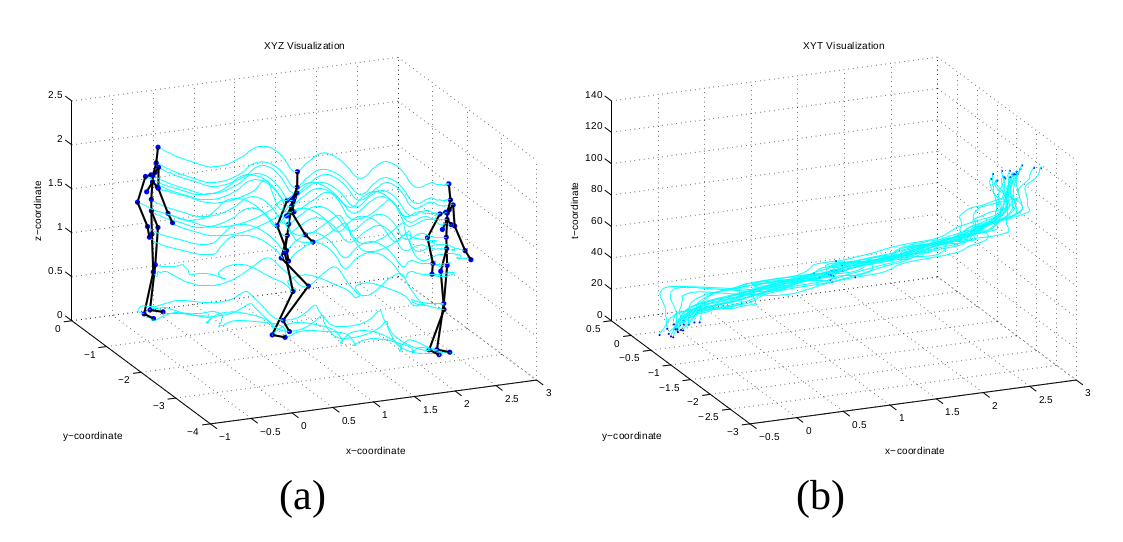
\includegraphics[width=\textwidth]{img_related/trajectories_sheikh}
    \caption{Tracking a person's joint positions to obtain motion trajectories for action recognition. \textit{(a)} XYZ space. \textit{(b)} XYT space. \cite{sheikh_exploring_2005}}
    \label{fig:trajectories_sheikh}
\end{figure}

Another class of hand-crafted feature approaches uses \textit{local space-time features}.
These approaches have emerged as the standard approach in video classification with manually engineered feature extractors \cite{karpathy_large-scale_2014}.
Local space-time features are descriptive video attributes, that are extracted from a local region of an input video, where sudden changes in motion appear (also called spatio-temporal interest points \cite{poppe_survey_2010}).
These points are considered highly informative for action recognition.

Generally local spatio-temporal feature approaches can be divided into three stages: \cite{karpathy_large-scale_2014}\cite{aggarwal_human_2011}
\begin{enumerate}
    \item \textbf{Feature Extraction}: Describes the process of determining where regions of motion are present and then transforming the raw RGB values around that region into a descriptive feature representation.
    Feature extraction can be further divided into the two sub stages interest-point detection and local description \cite{poppe_survey_2010}.
    \item \textbf{Feature Encoding}:
    Encoding all of the previously extracted features into a fixed-size video representation.
    Common representations are created using the bag-of-visual-words paradigm, the Fisher Vector\cite{perronnin_fisher_2007} or the Vector of Locally Aggregated Descriptors\cite{jegou_aggregating_2010}.
    \item \textbf{Classification}:
    Learns the correspondence between the video representations and the action class it contains.
\end{enumerate}

Prominent examples of approaches using local spatio-temporal features were proposed by \textcite{laptev_space-time_2005} and \textcite{dollar_behavior_2005}.
The approach of \cite{dollar_behavior_2005} incorporates a feature detector, that focuses on periodic motion.
A detected interest point is then described as a cube of video pixels called a \textit{Cuboid}.
The raw local pixel values of each cuboid are then further processed and aggregated into a global video representation.
Figure \ref{fig:dollar_cuboids} illustrates this approach.

\begin{figure}[H]
    \centering
    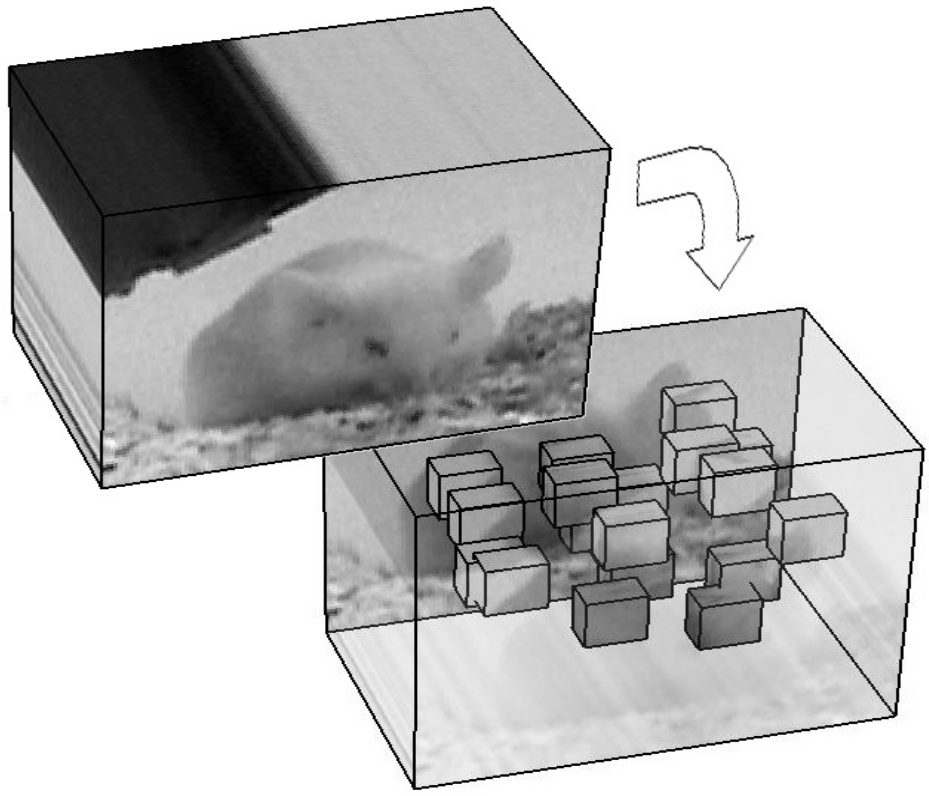
\includegraphics[width=0.4\textwidth]{img_related/dollar_cuboids}
    \caption{\cite{dollar_behavior_2005}}
    \label{fig:dollar_cuboids}
\end{figure}

A hybrid approach of using local spatio-temporal feature around previously sampled trajectories is proposed by \textcite{wang_action_2011}.
The approach is called \textit{Dense Trajectories} and is illustrated in figure \ref{fig:densetrajectories_approach}.
Instead of computationally costly feature detection, a dense number of points is sampled from the video's frames.
These points are then tracked along the temporal evolution of the video frames to capture the illustrated motion.
Local spatio-temporal feature are then extracted around the resulting trajectories and aggregated for action recognition.

\begin{figure}[H]
    \centering
    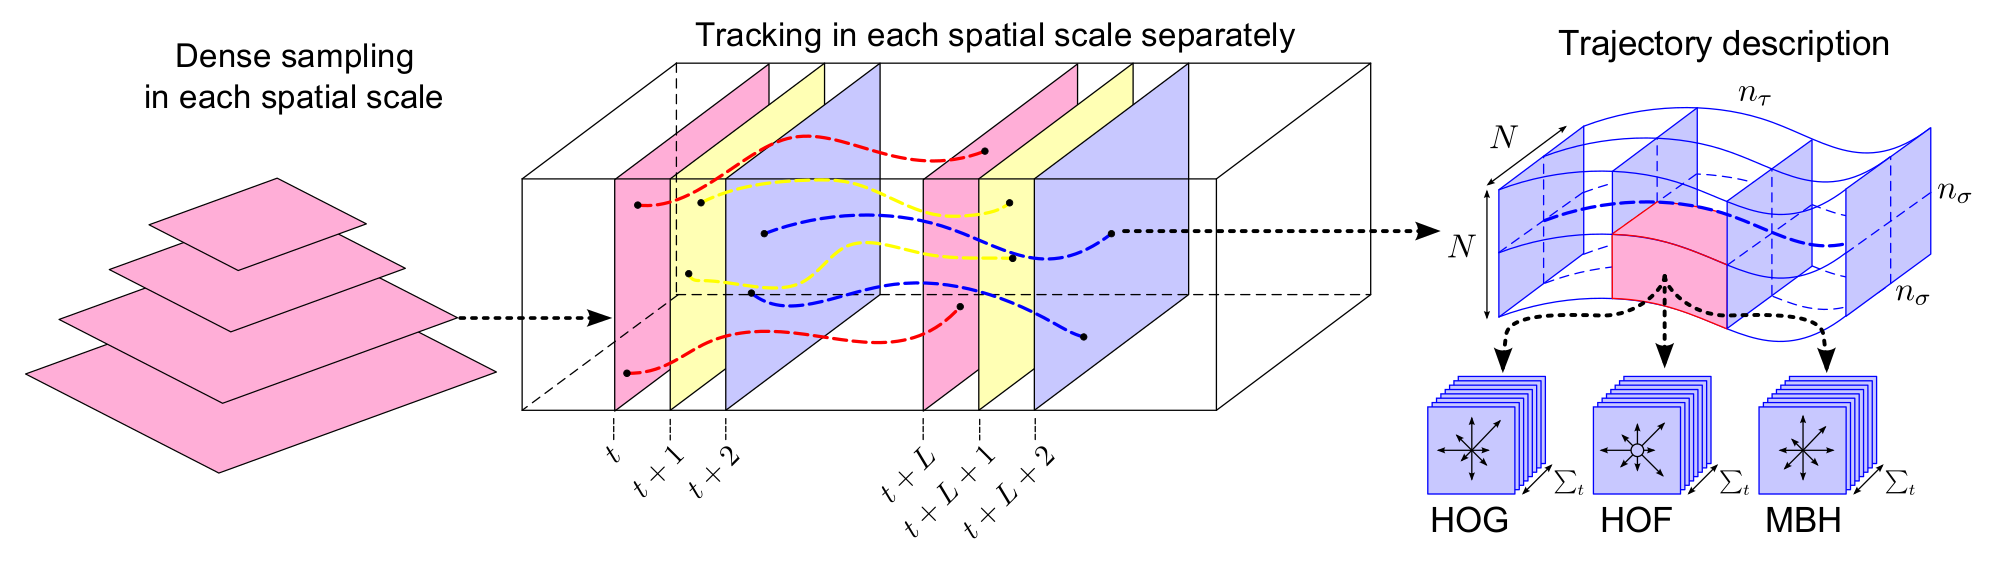
\includegraphics[width=\textwidth]{img_related/densetrajectories_approach}
    \caption{Description of densely extracted trajectories \cite{wang_action_2011}}
    \label{fig:densetrajectories_approach}
\end{figure}

Since background motion constitutes to the sampling of trajectories as well but does not convey any information about the performed action in the video, the approach was later extended to filter background motion by camera motion estimation\cite{wang_action_2013}.
The \textit{Improved Dense Trajectories} approach yielded state-of-the-art performance in action recognition by the time it was published. 

\subsection{Deep Learning Approaches}

Applying deep learning techniques to action recognition is motivated by the results that were achieved on other vision tasks. 
In contrast to hand-crafted feature-based methods, no manual feature engineering is required, because extracting features and encoding an input video into a descriptive representation can be learned from large amount of labelled training data.

Besides discriminative models such as convolutional neural networks, generative models are adopted for action recognition as well.
Examples include Convolutional Deep Belief Networks\cite{palasek_action_2016} and Recurrent LSTM Auto-encoders\cite{srivastava_unsupervised_2015}.
Generative models are particularly interesting for action recognition because they can be trained in an unsupervised way, i.e. with unlabelled input data.
Action recognition video datasets are generally harder to obtain, store and label than images, because they have bigger file sizes and an action in a video needs to be identified and temporally localized.

Using convolutional neural networks in action recognition can broadly be divided into two classes:
\begin{enumerate}
\item 3D CNNs are the natural extension from regular 2D CNNs to using three dimensional convolutional filters and thereby able to directly process spatio-temporal data, i.e. video volumes.
\item Two-stream network use regular 2D CNNs but process inputs in two separate streams.
A spatial stream processes raw RGB input frames, while an additional temporal stream processes direct motion information in the form of optical flow.
\end{enumerate}

\subsubsection{3D Convolutional Neural Networks}
An early approach to incorporate three dimensional convolutional kernels for action recognition has been proposed by \textcite{ji_3d_2013}.
The architecture still incorporates an initial hard-wired layer, i.e. fixed transformations to extract greyscale frames, frame gradients and optical flow along the horizontal and vertical axis.
Later models eliminate the first hard-wired through trainable layers and are considerably deeper.
This architecture, as illustrated in figure \ref{3dconv_architecture} contains $295,458$ trainable parameters in total.\footnote{For comparison: The \textit{C3D} model used in this work contains around $78,000,000$ parameters}.
The approach showed competitive results, but did not outperform the state-of-the-art at that time.

\begin{figure}[H]
    \centering
    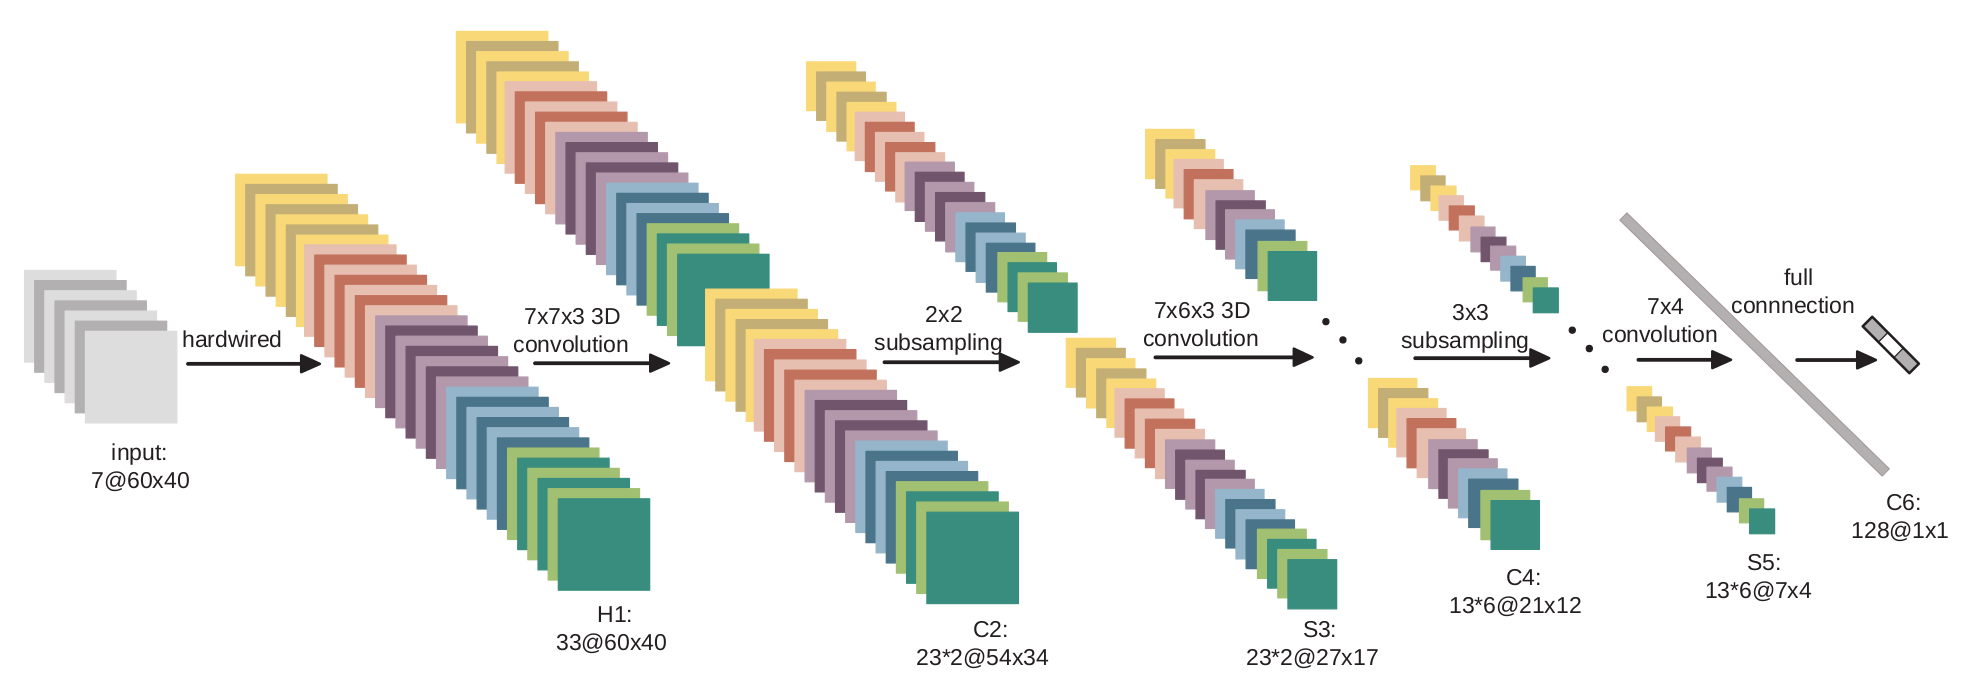
\includegraphics[width=\textwidth]{img_related/3dconv_architecture}
    \caption{Early 3D CNN for human action recognition \cite{ji_3d_2013}}
    \label{fig:3dconv_architecture}
\end{figure}

Building on the work of \textcite{ji_3d_2013}, follow-up approach of \textcite{baccouche_sequential_2011} addresses two main previous deficits.
That is \textit{(1)} the previous model still relies on a hand-crafted processing and \textit{(2)} only 15 frames were processed.
Therefore a 3D CNN without fixed pre-processing layers is used as a feature extractors and an LSTM was used to aggregate resulting clip representations to perform action recognition.

\begin{figure}[H]
    \centering
    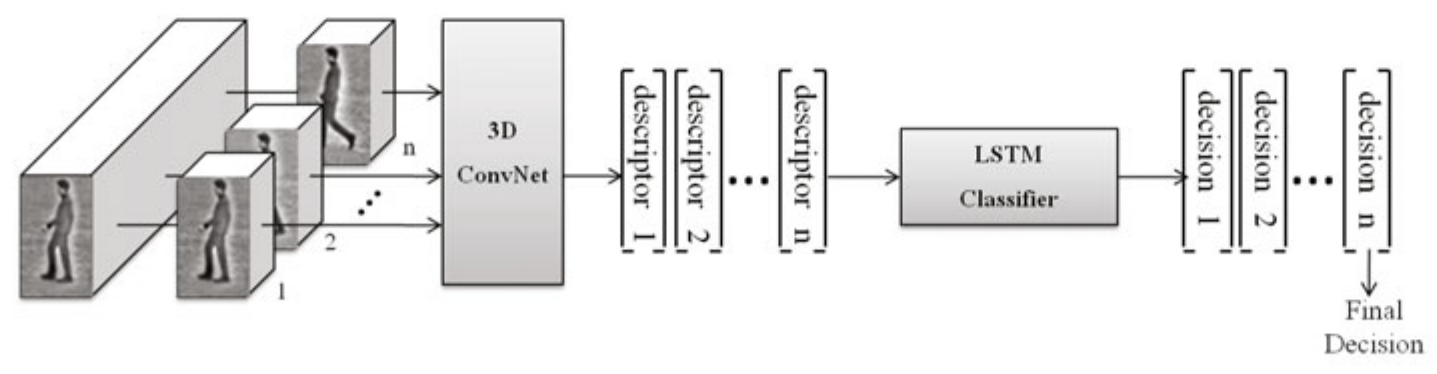
\includegraphics[width=\textwidth]{img_related/sequentialdeep_overview.png}
    \caption{3D CNN + LSTM architecture. \cite{baccouche_sequential_2011}}
    \label{fig:sequentialdeep_overview}
\end{figure}

This approach performs comparably to the one of \textcite{ji_3d_2013}.
Aggregating 3D CNN activations with an LSTM only results in a minor increase in accuracy, i.e. from $91.04\%$ to $92.17\%$ on the KTH dataset\cite{schuldt_recognizing_2004}.

\textcite{karpathy_large-scale_2014} perform a comprehensive evaluation on how to incorporate temporal information in convolutional neural network architectures in general.
The naive approach of simply classifying individual video frames and then averaging the results is compared to multiple different fusion techniques.
Using \textit{Late Fusion} two 2D CNNs are applied to two video frames with a fixed temporal distance between them.
An \textit{Early Fusion} approach incorporates 3D convolutions only in the first network layer and the \textit{Slow Fusion} approach is equivalent to general 3D CNNs.
The results show, that the \textit{Slow Fusion}, i.e. 3D convolutions in all network layers, performs best.
This work thereby backs up the use of 3D convolutions, which has among others motivated the development of the \textit{C3D} model (see section \ref{subsec:c3d}).

The work of \textcite{varol_long-term_2016} addresses similar to \textcite{baccouche_sequential_2011} a common deficit in 3D convolutional architectures for action recognition, namely that they process short, fixed-length video subsequences only.
Common temporal extends being learned from only span around 1-16 input frames at a time \cite{ji_3d_2013}\cite{karpathy_large-scale_2014}\cite{tran_learning_2015}.
The authors provide a systematical evaluation of the influence of temporal input length in 3D convolutional networks.
The used network architecture for evaluating temporal input lengths of $T = \{20, 40, 60, 80, 100\}$ frames is illustrated in figure \ref{fig:longterm_architecture}.

\begin{figure}[H]
    \centering
    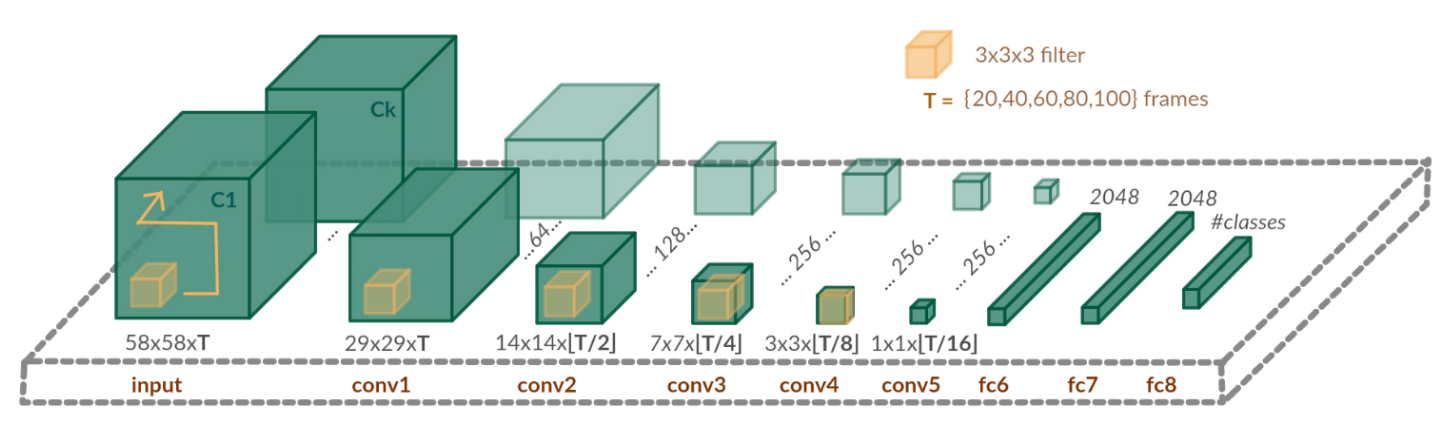
\includegraphics[width=\textwidth]{img_related/longterm_architecture}
    \caption{3D CNN architecture for evaluating the influence of the number of input frames on action recognition accuracy. \cite{varol_long-term_2016}}
    \label{fig:longterm_architecture}
\end{figure}

In order to process temporally longer inputs and not exceed computational limitations, the spatial resolution of inputs is decreased to either $58 \times 58$ or $71 \times 71$ pixel.
The results show, that incorporating temporally longer inputs for action recognition heavily improves the performance of the model.
On UCF-101 an increase of $+9\%$ recognition accuracy was achieved by extending the temporal input length from 16 to 60 frames.


\subsubsection{Two Stream Networks}
Two-stream convolutional neural networks for action recognition have to our best knowledge first been proposed by \textcite{simonyan_two-stream_2014}.
Due to their state-of-the-art performance, they have quickly been adapter by the action recognition community.
Two-stream networks are inspired by the human visual cortex, which according to \cite{goodale_separate_1992} contains two separate processing paths: One for static object recognition, and another independent one for guiding actions towards the recognized objects.

\textcite{simonyan_two-stream_2014} adapt this hypothesis in their neural network architecture for action recognition by implementing a spatial and a temporal stream.
The spatial stream processes raw RGB video frames, while the temporal stream receives stacked optical flow images in different channels.
The combined architecture is illustrated in figure \ref{fig:twostream_architecture}.

\begin{figure}[H]
    \centering
    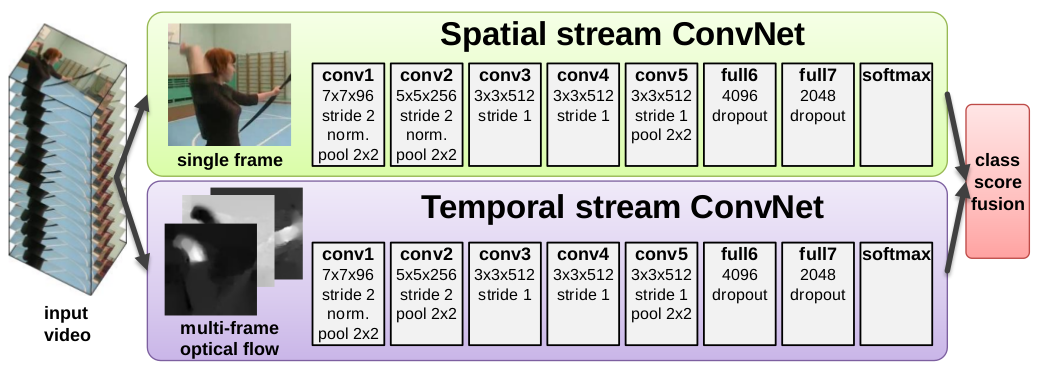
\includegraphics[width=0.9\textwidth]{img_related/twostream_architecture}
    \caption{Spatial stream and temproal stream network in the two-stream action recognition architecture by \textcite{simonyan_two-stream_2014}}
    \label{fig:twostream_architecture}
\end{figure}

Both streams are implemented as 2D CNNs.
The authors identify the advantage in separating the two streams in being able to pre-train the spatial network on large pre-existing image datasets such as ImageNet ??, since it is basically an image recognition architecture.
Both streams are fused late, after each network produced an individual class prediction.
The authors found fusing the class scores by an SVM works best and results in an accuracy of $88.0\%$ on UCF-101 and $59.4\%$ on HMDB-51.

As \textcite{baccouche_sequential_2011} and \textcite{varol_long-term_2016} addressed the deficit of short temporal input lengths in 3D CNNs, \textcite{ng_beyond_2015} address the same issue in the two-stream approach.
They aim at constructing a video representation in a two-stream setup from inputs with lengths in the order of tens of seconds.
The main idea is to apply multiple 2D CNNs to inputs in parallel, pooling the results and then merging them with the temporal stream.The number of applied CNNs thereby determines the processed input lengths.
To pool the CNN outputs, LSTMs or additional pooling are evaluated.
The approach is illustrated in figure \ref{fig:beyongshort_overview} and outperforms \textcite{simonyan_two-stream_2014} the original two-stream network by a small margin.

\begin{figure}[H]
    \centering
    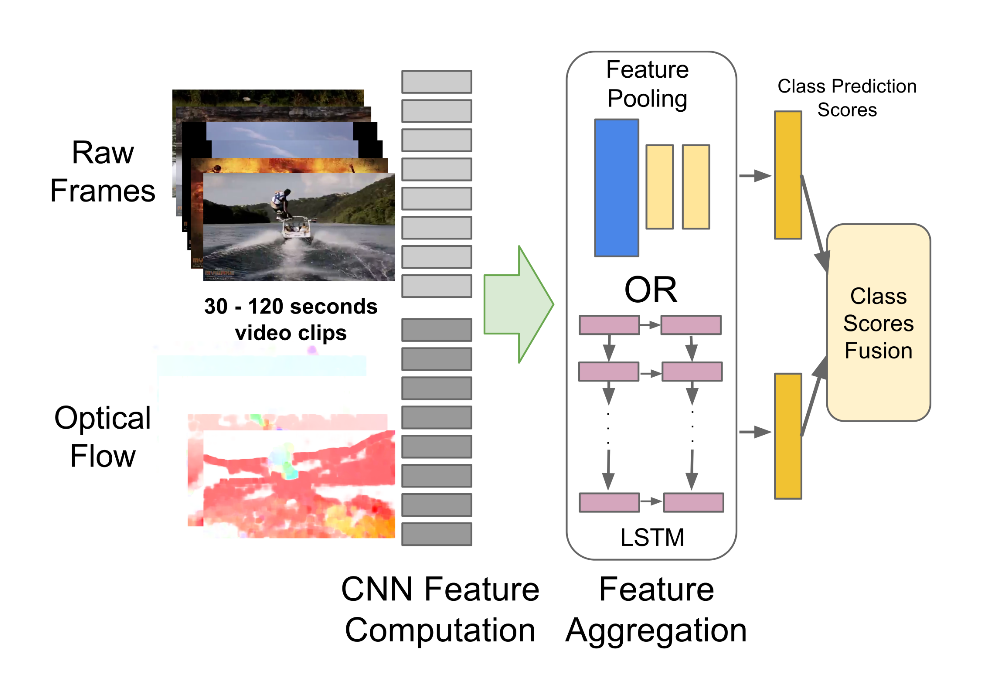
\includegraphics[width=0.8\textwidth]{img_related/beyondshort_overview}
    \caption{Approach to incorporate longer temporal inputs in a two-stream action recognition setup \cite{ng_beyond_2015}}
    \label{fig:beyondshort_overview}
\end{figure}

\textcite{feichtenhofer_convolutional_2016} aim at imporving the two-stream architecture by incorporating more sophisticated fusion strategies.
These include earlier fusion of the streams and keeping one of the streams after fusion, to re-fuse it again in the final layer.
These approaches are illustrated in figure \ref{fig:streamfusion_layerplacement}.

\begin{figure}[H]
    \centering
    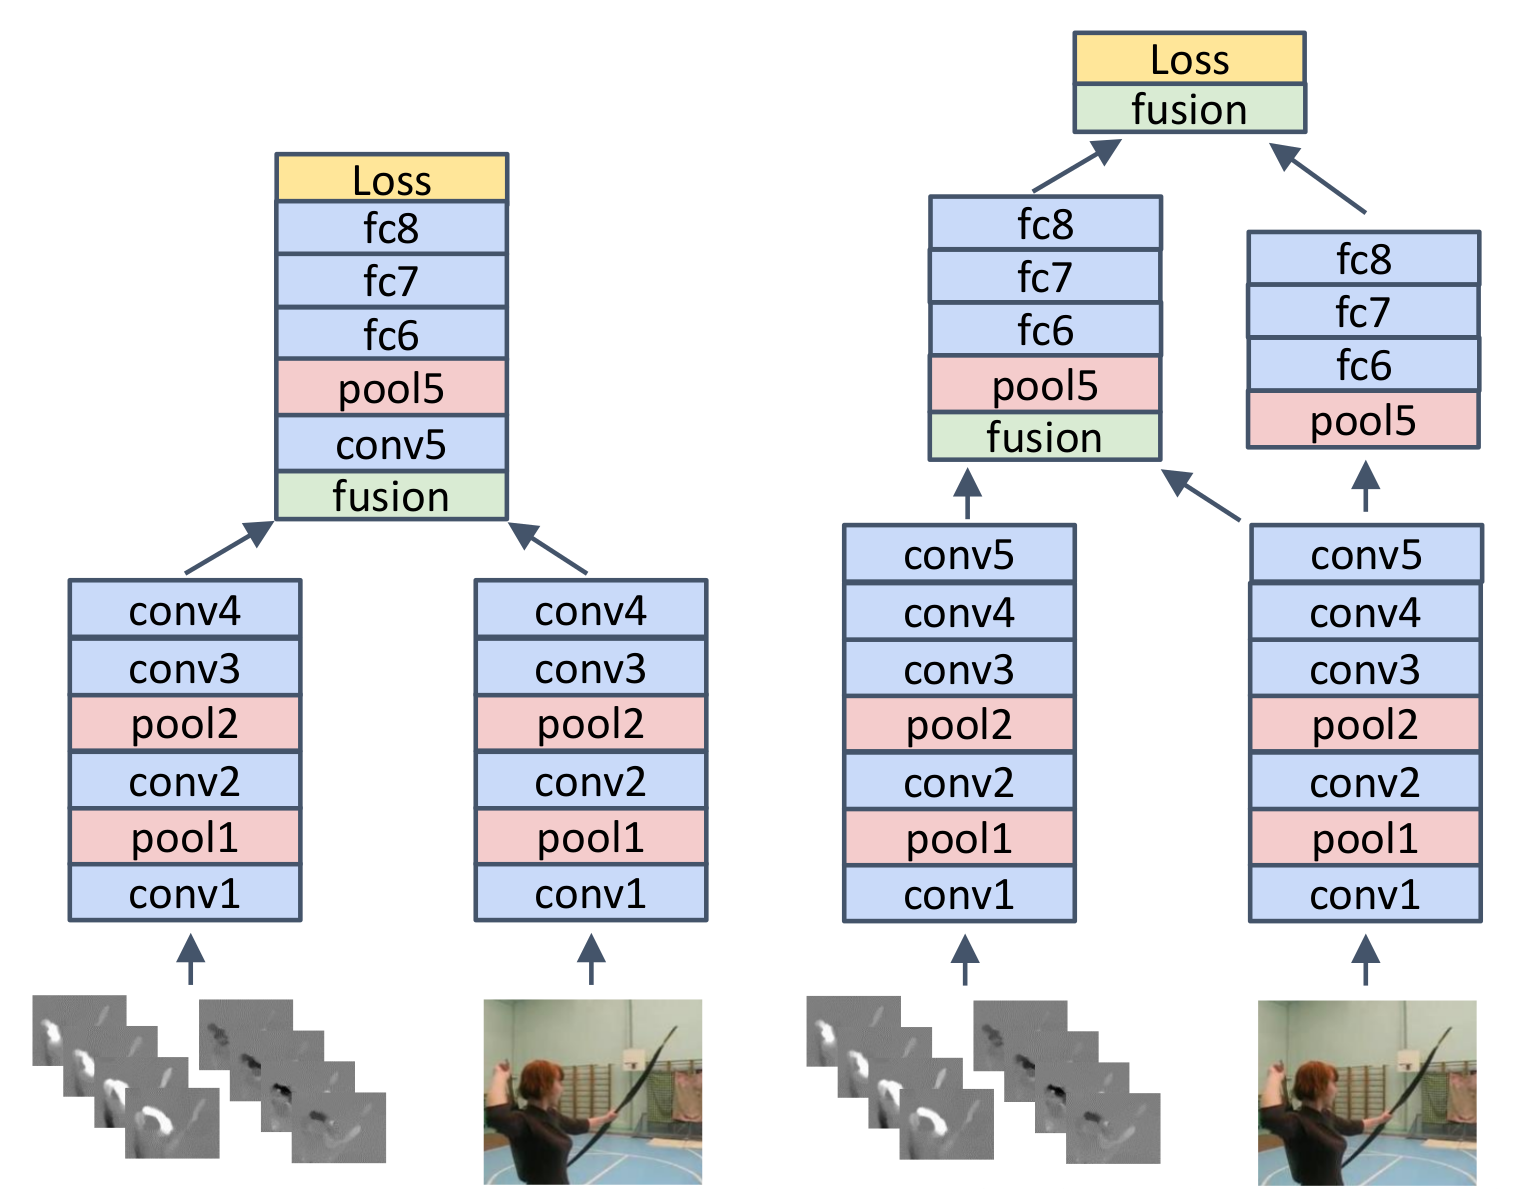
\includegraphics[width=0.75\textwidth]{img_related/streamfusion_layerplacement}
    \caption{  \cite{feichtenhofer_convolutional_2016}}
    \caption{Placement of fusion layers between the spatial and temporal stream in a two-stream architecture. (\textit{left}) Only the merged stream is kept. (\textit{right}) The spatial stream is maintained after first fusion operation and merged before the final layer. \cite{feichtenhofer_convolutional_2016}}
    \label{fig:streamfusion_layerplacement}
\end{figure}

Additionally several approaches of temporal fusion, i.e. incorporating the results of several temporally distant network inputs are being evaluated.
The authors identify an advantage of early network fusion: the number of parameter can be reduced by around a factor of 2.
The best performig temporal and spatial fusion approach results in an increase in performance of $+3.7\%$ with an significantly descreased number of network parameters.


\subsubsection{Hybrid Approaches}
\textcite{wang_action_2015} extend the hand-crafted feature-based approach using \textit{Dense Trajectories} by \textcite{wang_action_2013} with deeply learned features of two-stream CNNs \cite{simonyan_two-stream_2014}.
The approach is called \textit{Trajectory-pooled Deep Convolutional Descriptors (TDD)}.
A two-stream CNN is first trained on a large dataset as in \cite{simonyan_two-stream_2014}.
Dense trajectories are then extracted from input videos \cite{wang_action_2013} to identify regions of motion.
The previously trained two-stream CNN functions as a generic feature extractor instead of using hand-crafted feature extractors, to obtain discriminative features around the sampled trajectories.
These features are then aggregated over the whole video using the Fisher Vector representation \cite{sanchez_image_2013} and classified with an SVM.

Another successful hybrid approach of combining a two-stream architecture with 3D convolutions was recently published by \textcite{carreira_quo_2017}.
The authors use a pre-trained 2D CNN, i.e. the Inception-V1 model \cite{szegedy_going_2015-1} pre-trained on ImageNet and extend it to process spatio-temporal input data.
Extending is done by \textit{inflating}\textcite{carreira_quo_2017} the model, i.e. each 2D convolution and pooling kernel is replicated along an additional third dimension.
The authors note, that the inflated 3D model is already properly initialized from the pre-trained weights of the 2D kernels.


\subsection{C3D}
\label{subsec:c3d}
The work of \textcite{tran_learning_2015} provides a prominent example of a 3D convolutional architecture, which does not require the explicit calculation of optical flow.
Optical flow has previously been incorporated in an additional temporal network stream by \textcite{simonyan_two-stream_2014}.
The network in \cite{tran_learning_2015} uses a volume of stacked video frames as input and therefore performs action recognition on raw RGB inputs only.
By training the network on the very large noisily labelled dataset Sports-1M \cite{karpathy_large-scale_2014}, the authors were able to train a generic spatio temporal feature extractor, which they call \textit{C3D}.
That is, the activations of the network's last fully connected layer can be used as a generic feature representation of the input.
An arbitrary classifier can then be trained on this input-representation to perform several different video-based vision tasks such as action recognition, scene classification or object detection.

The work of \textcite{karpathy_large-scale_2014} motivated the incorporation of 3D convolutions in \textit{C3D} by providing a comparative evaluation on different fusion strategies, i.e. on how to combine temporal and spatial information in different neural network architectures.
\textcite{tran_learning_2015} additionally conclude, the advantageous property of 3D convolutions, that temporal information is not immediately but gradually condensed along the layer of a 3D CNN.

\begin{figure}[H]
    \centering
    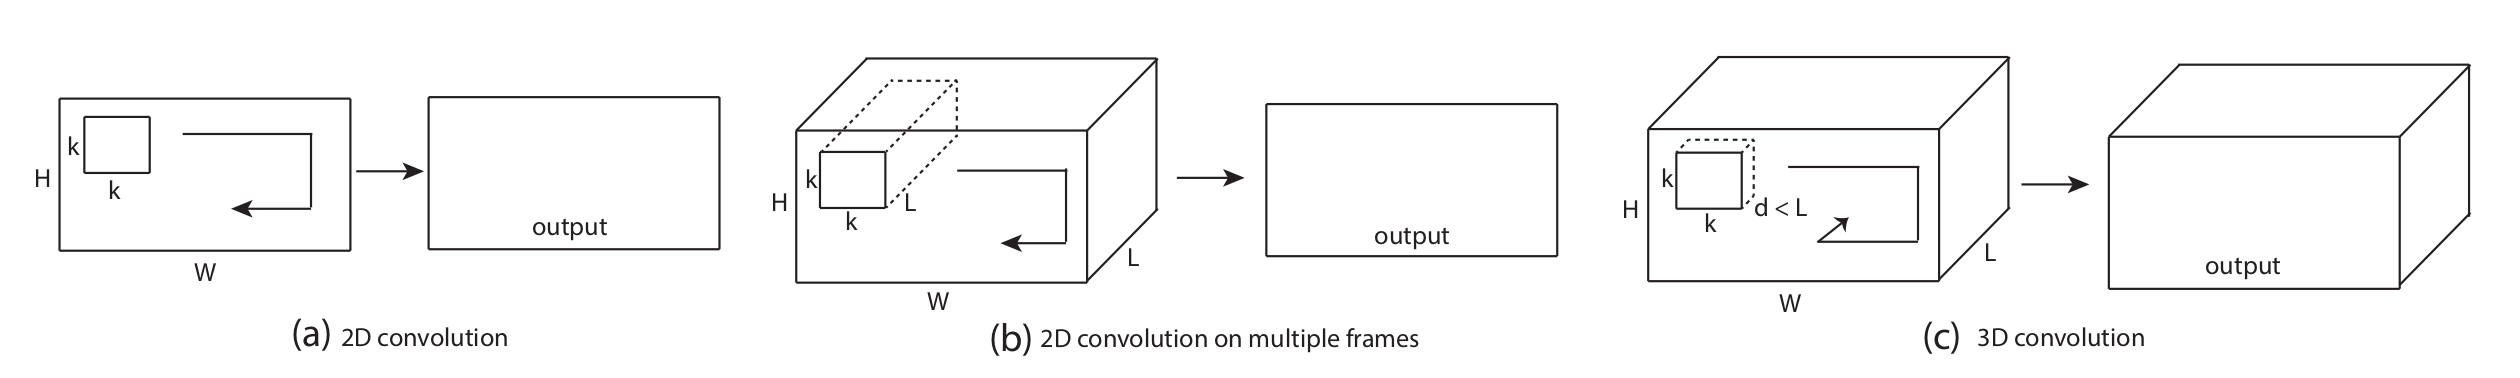
\includegraphics[width=\textwidth]{img_related/c3d_2dconv3dconv}
    \caption{Preservation of the temporal dimension by 3D convolutions: \textit{(a)} and \textit{(b)} 2D convolutions on a single or multiple frames results in a 2D feature map without temporal dimension. \textit{(c)} 3D convolutions on multiple input frames preserves the temporal dimension and results in a 3D feature map. \cite{tran_learning_2015}}
    \label{fig:c3d_2dconv3dconv}
\end{figure}

\textcite{tran_learning_2015} initially perform experiments on the smaller action recognition dataset UCF-101 \cite{soomro_ucf101:_2012}, to find the optimal size of kernels for the \textit{C3D} architecture. Results indicate, that kernels of size $3 \times 3 \times 3$ perform best.
The final architecture consists of 8 3D convolutional layers, 5 max-pooling layers, two fully-connected layers and a softmax output layer.
The architecture and layer sizes are illustrated in figure \ref{fig:c3d_architecture}.

\begin{figure}[H]
    \centering
    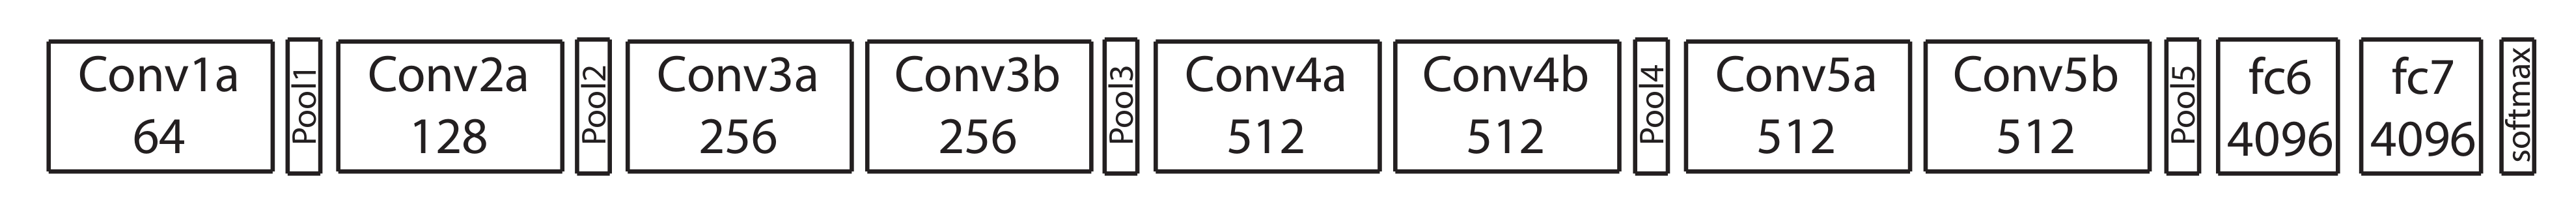
\includegraphics[width=\textwidth]{img_related/c3d_architecture}
    \caption{C3D architecture. Number of filters is given in each box. \cite{tran_learning_2015}}
    \label{fig:c3d_architecture}
\end{figure}

Final results when using a single \textit{C3D} network yield an accuracy of $82.3\%$ on UCF-101 \cite{soomro_ucf101:_2012}.
Note that these results were obtained from classifying the activations of the network's last fully-connected layer with an SVM.
The network was trained on the very large Sports-1M dataset \cite{karpathy_large-scale_2014} for this evaluation.
Only training the SVM on top of the networks activations uses the UCF-101 dataset.

Due to its competitive performance, the \textit{C3D} network is used as a prominent example of a 3D convolutional neural network using only raw RGB inputs.
\textcite{carreira_quo_2017} use it as main architecture to compare their own approach against.
Although the results of \textit{C3D} are competitive, the prototypical two-stream approach by \textcite{simonyan_two-stream_2014} outperforms \textit{C3D} by yielding $88.0\%$ accuracy on UCF-101.
Two-stream approaches are therefore considered the more successful architectures in action recognition \cite{wang_action_2015}, since they treat the spatial and temporal dimension differently.


\subsection{Temporal Order Verification}
\label{subsec:tov}

The work of \textcite{misra_shuffle_2016} is most related to ours.
The authors incorporate \textit{Temporal Coherency} between video frames to learn image representations, which are highly discriminative towards motion and therefore well suited for Action Recognition.
Our work is the logical continuation from learning these action representations with 2D CNNs as in \cite{misra_shuffle_2016} to 3D CNNs.

\textit{Temporal Coherency} describes an inherent relation between consecutive video frames.
More precisely, consecutive frames are semantically and dynamically correlated \cite{herath_going_2016}.
This means in terms of action recognition: Two consecutive frames are highly likely to present the same action and are limited by the laws of physics in the magnitute of change that can occur between them.

\textit{Temporal Coherency} can be used as a weak form of supervision in training deep networks, in contrast to strong supervision regular semantic labels.
\textcite{misra_shuffle_2016} propose an auxiliary quasi-unsupervised pre-training method which incorporates this \textit{Temporal Coherency} by first training a network on a binary classification task.
More precisely: The Network is presented with a sequence of input frames, which may have been randomly permuted, and has to determined if the sequence is in correct temporal order or not.
This pre-training task is called \textit{temporal order verification}.

This is, in the strictest sense, not an unsupervised training task, but since obtaining the label (\textit{correct temporal order} or \textit{incorrect temporal order}) is free, the authors attribute it as unsupervised \cite{misra_shuffle_2016}.
This has the advantage, that easily obtainable unlabelled data can be used for pre-training the network.

\textcite{misra_shuffle_2016} evaluate their approach by presenting three video frames to a triplet siamese CNN with 2D convolutions (see figure \ref{fig:shufflelearn_approach}).
Their results show, that using four or five frames did not result in an increase of performance.
Datasets utilized for training and evaluation are UCF-101 \cite{??} and HMDB-51 \cite{??}

\begin{figure}[H]
    \centering
    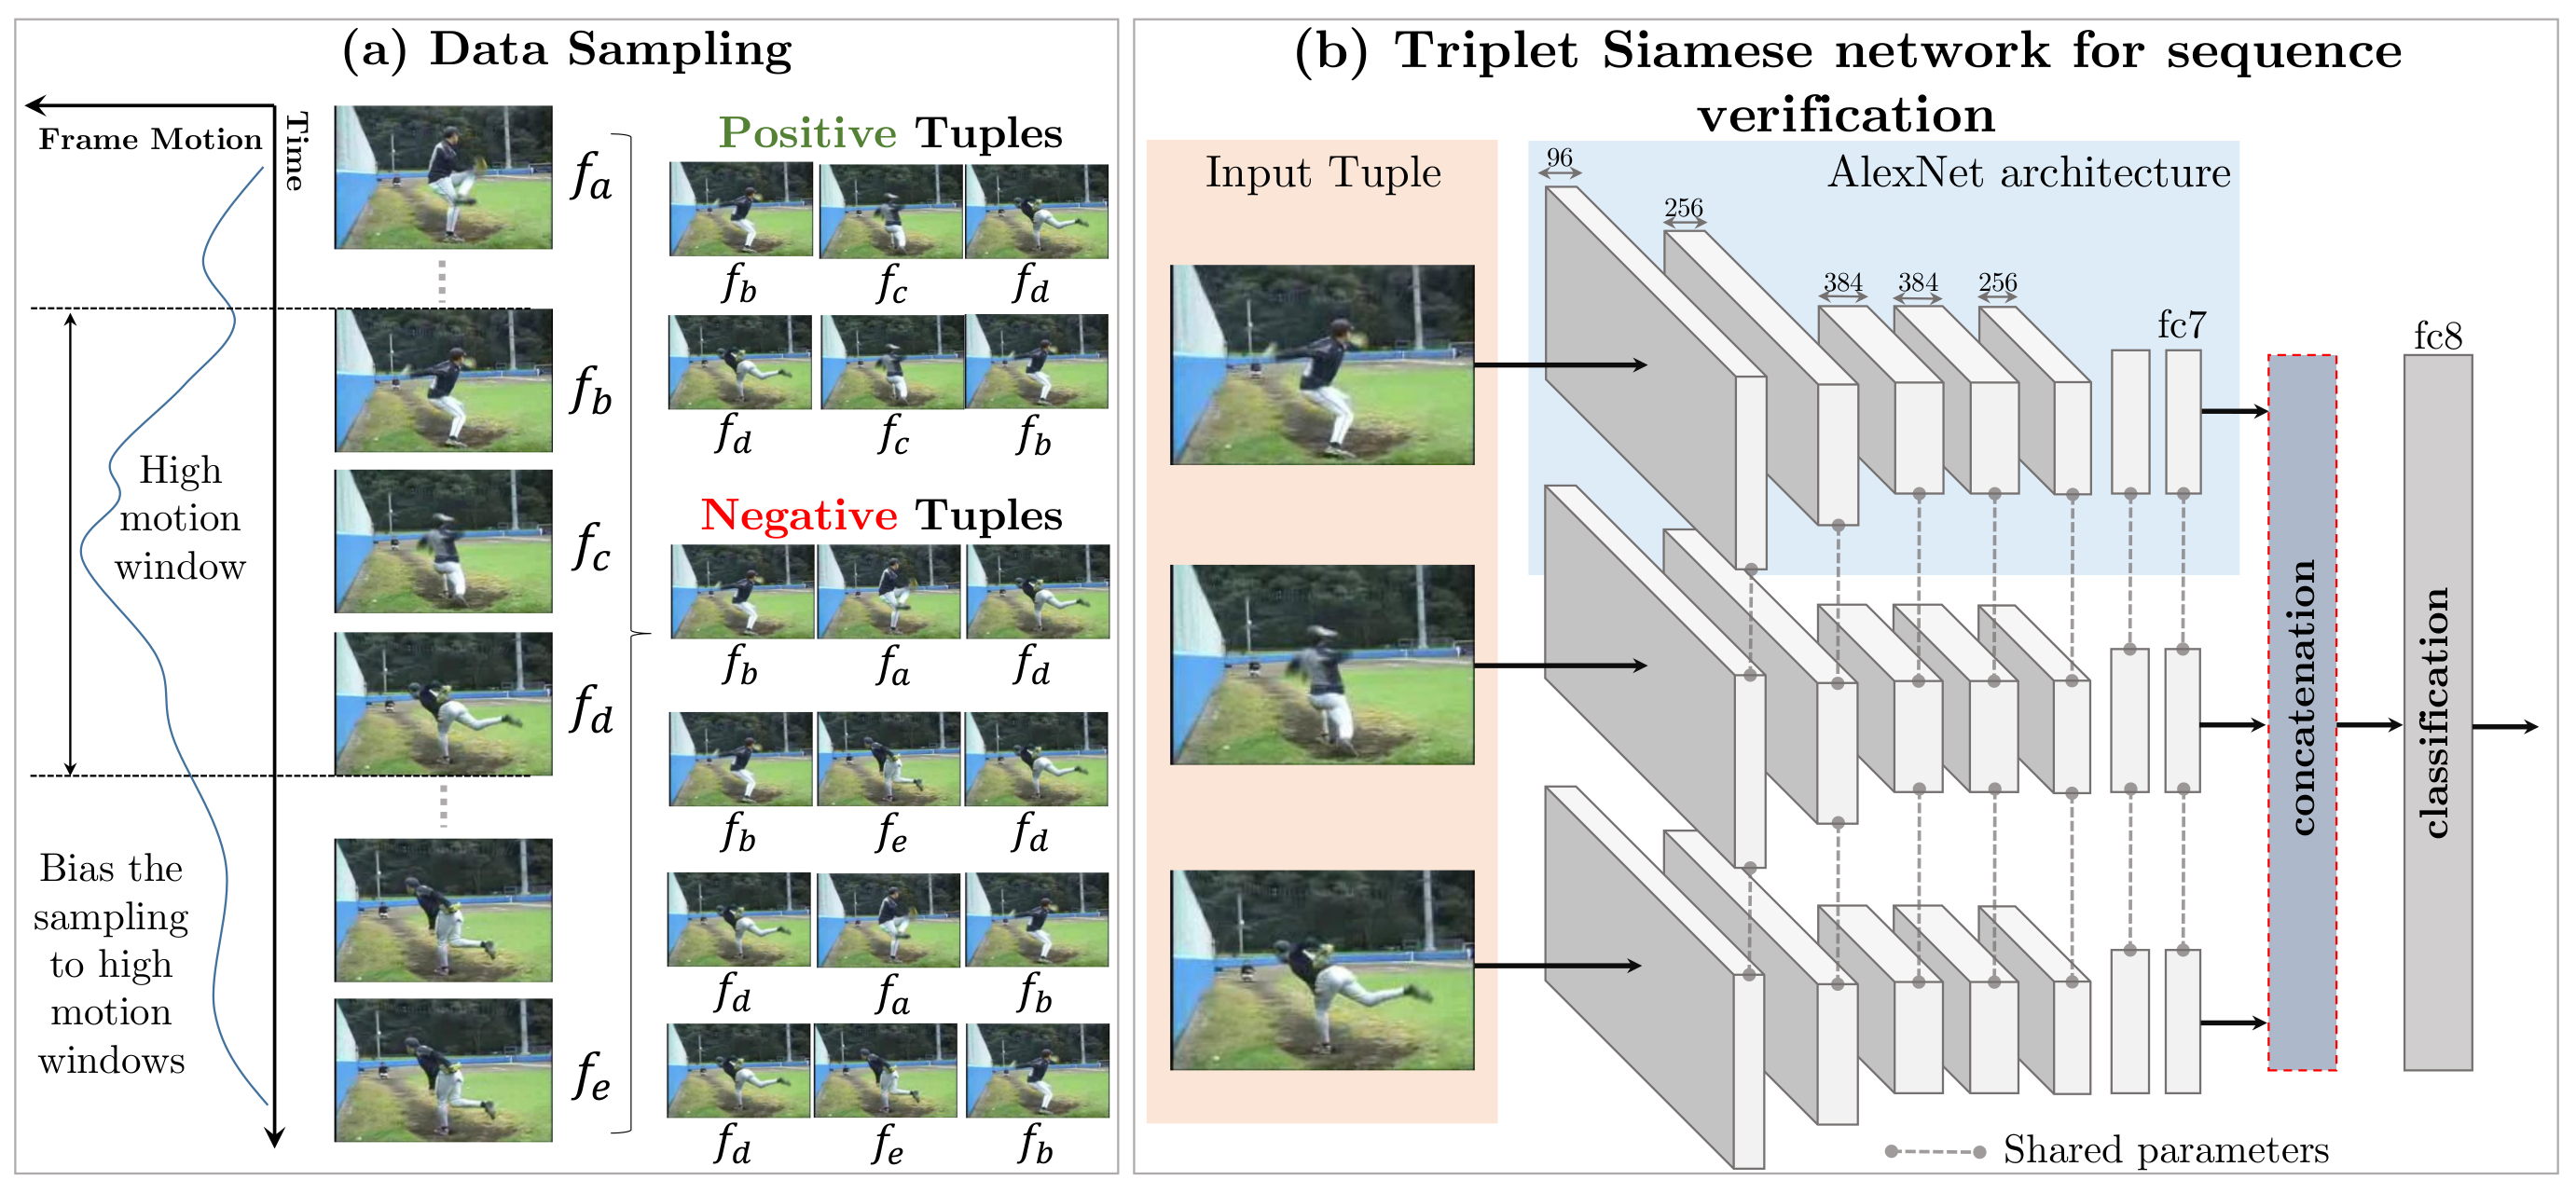
\includegraphics[width=\textwidth]{img_related/shufflelearn_approach}
    \caption{\textit{(Left)} Sampling of input sequences during temporal order verification. Sampling was biased towards regions with motion present in order to not obtain too similar frames. \textit{(Right)} Triplet siamese convolutional neural network, with shared weights. \cite{misra_shuffle_2016}}
    \label{fig:shufflelearn_approach}
\end{figure}

The authors use optical flow between two frames \cite{farneback_two-frame_2003} to identify a high motion window in the input video and construct positive examples (\textit{correct temporal order}) and negative examples (\textit{incorrect temporal order}) from the frames contained in it.
This ensures a certain magnitude of motion between the sampled frames and results in frame tuples, which are clearly distinguishable when permuted.

More precisely: Five frames $\{f_a, f_b, f_c, f_d, f_e\}$ are sampled from an input video, with $a < b < c < d < e$.
Out of these $f_a, f_b, f_c$ need to lie in the high motion window.
$f_b$ and $f_d$ are taken as start and end of the input sequence.
To construct a negative example (\textit{wrong temporal order}), $f_e$ or $f_a$ are inserted as middle frame to complete the input sequence.
The authors note, that it is vital to keep $f_b$ and $f_d$ as beginning and end of the input, i.e. the correct frames of the middle triple.
A mere inversion, i.e. $f_d, f_c, f_b$ is used as positive examples.

The incorporated network is available in the Caffe-Framework \cite{jia_caffe:_2014-1} and is called CaffeNet, an adapted version of the AlexNet model \cite{krizhevsky_imagenet_2012-1}.
The CNN model is arranged as a siamese triplet, with weight sharing.
That is: three identical copies of the network model each process one input frame, the results activations of the fully-connected layer are concatenated and then classified by an additional fully connected layer.
The individual network models share weights, i.e. each of them receive the same weight updates.

Results are obtained by training the composite model on UCF-101 and HMDB-51.
The model is either trained from scratch (weights are randomly initialized), pre-trained with \textit{temporal order verification} (weights are initialized from a pre-trained model) or pre-trained on UCF-101 for the evaluation on HMDB51.

\begin{table}[H]
    \centering
    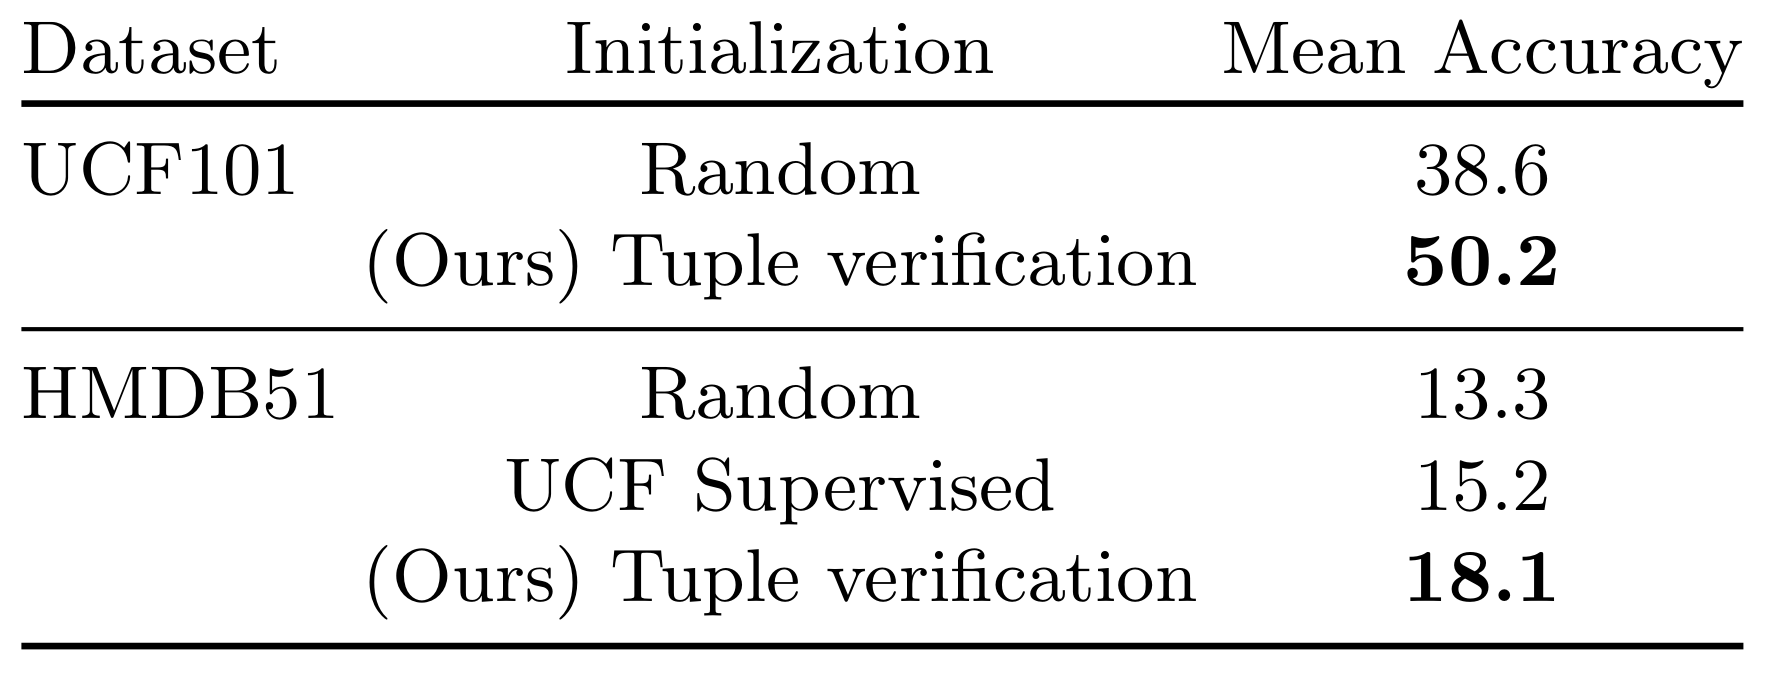
\includegraphics[width=0.6\textwidth]{img_related/shufflelearn_results}
    \caption{Perfomance gain in mean accuracy when incorporating temporal order verification as weight-initialization method on UCF-101 and HMDB-51 \cite{misra_shuffle_2016}}
    \label{tab:shufflelearn_results}
\end{table}

Table \ref{tab:shufflelearn_results} shows the increase in final performance after fine-tuning the model on either UCF-101 or HMDB-51.
The increase in performance of $+11.6\%$ is most prominent on UCF-101.
On HMDB-51 initializing the model using \textit{temporal order verification} achieves an increase in accuracy of $+4.8\%$, which is smaller than on UCF-101 but still significant.
Notably initialization from \textit{temporal order verification} outperforms initiliazing the network from regular pre-training on labeled data.
\bigskip

\textbf{Implementational details:}\\
\begin{itemize}
    \item The authors did not use any additional unlabeled data for pre-training, but sample around $900$k triples for \textit{temporal order verification} from the labeled datasets itself.
    \item Weights are randomly initialized for the \textit{temporal order verification} pre-training. 
    \item Pre-training is conducted for $100$k iterations with a fixed learning rate of $10^{-3}$ and a batch-size of 128 tuples (This results in around $14$ epochs in total for a pre-training set of $900$k triples).
    \item Best results were obtained with $25\%$ positive and $75\%$ negative triples.
    \item Batch normalization \cite{ioffe_batch_2017} is used during training.
    \item A single CaffeNet model is then initialized from the weights obtained from pre-training the siamese triplet. It is trained for $20$k iterations with a batch size of $256$ frames on UCF-101 and HMDB-51.
    \item The learning rate used for fine-tuning the model $10^{-2}$, which is decayed to $10^{-3}$ after $14$k iterations.
    \item Evaluation results are obtained from averaging random crops and flips from each test-video. First $25$ frames are uniformly sampled per video, $5$ input-sized regions are cropped out and flipped. This results in a total of $250$ inputs for averaging per video ($25$ frames $\times$ $5$ crops $\times$ $2$ flips).
\end{itemize}
